\section{Which ingredient does what}\label{sec:ablations}

The method combines pooling, regimes, and adaptivity; a reader
should know what each buys. Figure~\ref{fig:decomposition} and
Table~\ref{tab:ablations} decompose stress coverage across the reduction
grid of Section~\ref{sec:method}; the summary is that
\emph{pooling carries the average, regimes carry the conditional
structure}.

\begin{figure}[t]
\centering
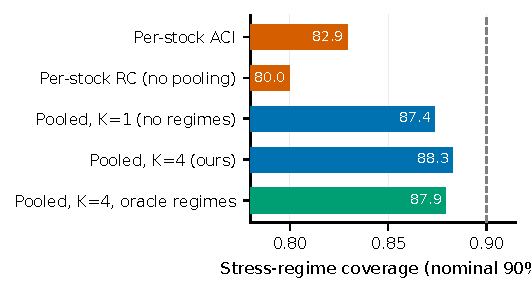
\includegraphics{figures/fig_decomposition.pdf}
\caption{Mechanism decomposition: stress-regime coverage as
ingredients are added. Pooling the cross-section closes most of the
average gap; regime conditioning adds the remainder on this slice;
its distinctive contributions are conditional (see text). Hindsight regimes
(full-sample smoothed memberships, deliberately noncausal) sit 0.2
points above the causal filtered HMM and do not exceed the causal
bins.}
\label{fig:decomposition}
\end{figure}

\begin{table}[t]
\centering
\caption{Ablations: stress coverage and width under reductions of
the full method. All rows use the zero-tuning adaptive configuration on
the pool forecast unless stated.}
\label{tab:ablations}
\small
\begin{tabular}{lcc}
\toprule
Configuration & Stress coverage & Stress width \\
\midrule
Per-stock (no pooling) & .800 & 1.70 \\
Pooled, $K=1$ (no regimes) & .875 & 2.26 \\
Pooled, $K=2$ & .883 & 2.33 \\
Pooled, $K=4$ (canonical) & .883 & 2.33 \\
Pooled, $K=4$, + per-stock offsets & .883 & 2.33 \\
Pooled, $K=4$, forecaster = HAR & .884 & 2.27 \\
Pooled, $K=4$, forecaster = LightGBM & .883 & 2.26 \\
\bottomrule
\end{tabular}
\end{table}

\paragraph{Pooling is the big lever for averages.} A single stock visits
the stress regime too rarely to calibrate itself: per-stock calibration
reaches 80.0\% stress coverage; pooling the cross-section under one
marginal tracker ($K = 1$) reaches 87.5\%. This ordering is worth stating
directly because it is not the usual sales pitch: the cross-section, not
the regime label, supplies most of the raw coverage repair.

\paragraph{What pooling actually is.} Because the pooled update sums
errors over $\sim$100 stocks, it confounds two channels: sharing one
threshold across the cross-section, and mechanically moving
$\sim$100$\times$ further per day. Table~\ref{tab:mechanism} separates
them with fixed-rate arms in a $2 \times 2$ over \{pooled, per-stock\}
$\times$ \{fast, slow\} effective daily rate, plus an averaged-error
arm. Three findings. First, summing versus averaging the cross-sectional
error is pure rescaling (stress coverage .841 vs .843). Second, the
average-coverage channel is the \emph{effective daily step}: a slow
pooled tracker fails exactly like a slow per-stock tracker (.770 vs
.770), and a per-stock tracker granted the pooled tracker's daily speed
matches its average stress coverage (.840 vs .841), consistent with the
strong cross-sectional dependence anticipated in
Remark~\ref{rem:dependence}: one hundred correlated stock-days do not
carry one hundred days of information.

\paragraph{Fast rates are necessary but not sufficient.} The required
per-stock rate ($\approx 0.2$ per observation) exceeds the standard
expert grid's maximum of $0.064$, which raises the obvious objection:
perhaps the headline gap exists only because the per-stock baselines
were denied the rates they needed. Table~\ref{tab:expgrid} closes this
question by extending the grid to $0.512$ and rerunning every
configuration. The per-stock aggregator \emph{does} find and use the
fast rates --- its issued effective rate on stress days rises from
$0.03$ to $0.17$ --- and its stress coverage improves from 80.0\% to
83.7\%, recovering roughly half the deficit. But it remains $4.6$
points below RC ($t = 4.8$, $p < .001$, date-clustered), and the same
pattern holds for every other fast-rate route: DtACI with its
learning-rate grid widened from $0.2$ to $0.8$ reaches 85.4\%
($-2.7$, $p = .04$); a pooled tracker stepping once per day on the
cross-sectional \emph{average} error, with the identical per-day rate
menu as the per-stock arms, reaches 84.8\% ($-3.3$, $p < .001$).
Meanwhile the headline method is insensitive to the extension: 88.3\%
under either grid ($p = .99$). The interpretation is variance, not
speed alone: a single stream updated at rate $0.2$ tracks its own
noise, whereas the pooled update applies one summed cross-sectional
mini-batch step per day --- the same daily movement driven by the
average of $n_t$ error indicators. How much variance that averaging
removes is bounded by cross-sectional dependence: for exchangeable
errors with pairwise correlation $\rho$,
$\operatorname{Var}(n^{-1}\sum_i u_i) = \sigma^2[\rho + (1-\rho)/n]$,
which floors at $\rho\sigma^2$ rather than falling as $1/n$, so the
effective panel size is $n_{\mathrm{eff}} = n / (1 + (n-1)\rho)$. We
estimate $\rho$ of the daily upper-miss indicators and the implied
$n_{\mathrm{eff}}$, and probe the same question in controlled
simulations varying $\rho$, panel size, and heterogeneity
(Section~\ref{sec:mechanism-sims}): the variance reduction pooling
delivers is that of $n_{\mathrm{eff}}$ conditionally independent
streams, material but far short of $\bar n$. Pooling's operative
contribution is that the summed mini-batch update supplies the
panel-scaled rate and this dependence-limited variance reduction
automatically, inside a standard specification; the shared threshold
additionally tightens the cross-sectional coverage distribution
(Table~\ref{tab:perstock}).

\begin{table}[t]
\centering
\caption{Expanded rate grid: giving the baselines the fast rates.
``Std'' grids end at 0.064 (panel machinery) or 0.2 (DtACI, raw-score
scale); ``exp'' grids add 0.128/0.256/0.512 (or 0.4/0.8 for DtACI). All
arms adaptive, full panel; the difference column is the date-clustered
paired stress-coverage test against RC (std grid). ``Eff.\ rate'' is the
issued effective per-observation rate on stress days.}
\label{tab:expgrid}
\small
\begin{tabular}{lccccc}
\toprule
Arm & Grid & Stress cov. & Diff.\ vs RC & $p$ & Eff.\ rate \\
\midrule
RC ($K=4$, pooled, summed) & std & .883 & --- & --- & .010 \\
RC ($K=4$, pooled, summed) & exp & .883 & $-$0.0 & .99 & .021 \\
Pooled $K=1$ & exp & .873 & $-$0.9 & .43 & .033 \\
Pooled $K=4$, averaged errors & exp & .848 & $-$3.3 & $<.001$ & .244 \\
Per-stock $K=4$ & std & .800 & $-$8.3 & $<.001$ & .029 \\
Per-stock $K=4$ & exp & .837 & $-$4.6 & $<.001$ & .175 \\
Per-stock $K=1$ & exp & .843 & $-$3.9 & .005 & .136 \\
DtACI (per stock, raw scores) & exp & .854 & $-$2.7 & .04 & --- \\
\bottomrule
\end{tabular}
\end{table}

\begin{table}[t]
\centering
\caption{Pooling-mechanism identification. All arms fixed-rate
(no adaptivity), $K = 4$ bins, full panel. ``Fast'' arms move an
effective $\approx 0.2$ per day (the pooled tracker's speed); ``slow''
arms $\approx 0.002$.}
\label{tab:mechanism}
\small
\begin{tabular}{lccc}
\toprule
Arm & Stress coverage & Marginal & Width \\
\midrule
Pooled, summed errors (fast) & .841 & .896 & 1.67 \\
Pooled, averaged errors (fast) & .843 & .896 & 1.67 \\
Pooled, rate $/\,100$ (slow) & .770 & .866 & 1.49 \\
Per-stock, standard rate (slow) & .770 & .858 & 1.52 \\
Per-stock, rate $\times\,100$ (fast) & .840 & .895 & 1.70 \\
\bottomrule
\end{tabular}
\end{table}

\subsection{Effective panel size and simulations}
\label{sec:mechanism-sims}

The variance argument above depends on how correlated the panel's miss
indicators actually are, so we estimate it. Using the moment identity
$\operatorname{Var}(\bar u_t) = \sigma^2[\rho + (1-\rho)/n]$ on the
daily upper-miss indicators of the headline run, the intra-date
correlation is $\rho = .16$ over all days --- an effective panel size
$n_{\mathrm{eff}} \approx 6$, a material but far-from-$\bar n$
variance reduction --- and $\rho = .90$ on stress days, an effective
panel size of $\approx 1.1$: on crisis days the cross-section misses
together, and the panel is informationally close to a single stream.
This sharpens the mechanism decomposition. In regime interiors and
transitions in aggregate, pooling supplies both the panel-scaled rate
and a genuine (sixfold) variance reduction; \emph{within} acute stress
the variance channel is nearly absent, and pooling's residual advantage
over rate-matched per-stock arms (Table~\ref{tab:expgrid}) must come
from the graded batch signal --- the daily miss \emph{fraction} across
$\sim$100 stocks is a finer gradient than one stock's binary miss ---
and from the shared threshold itself.

Controlled simulations isolate what the empirical ablations confound.
On synthetic factor-structured panels ($s_{it} = \sqrt{\rho} f_t +
\sqrt{1-\rho}\, e_{it}$, stress scale $\times 3$, two-state Markov
regimes with stationary stress probability $.05$, per-stock scale
heterogeneity $\sigma_h$, all trackers at the same fixed rate so speed
is controlled), the pooled regime-conditional tracker dominates
per-stock and pooled-marginal trackers in every cell of a $\rho \in
\{0, .3, .6, .9\} \times n \in \{10, 100\} \times \sigma_h \in
\{0, .5\}$ grid, and its advantage behaves exactly as the dependence
formula predicts: largest at $\rho = 0$ with $n = 100$ (stress
coverage $.83$ vs $.51$ per stock), shrinking monotonically in $\rho$
(to $.67$ at $\rho = .9$) and eroded by heterogeneity at low $\rho$.
Pooling helps most when the cross-section is large, weakly dependent,
and homogeneous; it never hurt in these designs, but its margin is
governed by $n_{\mathrm{eff}}$, not $n$. Full grids are in the
replication artifacts.

\paragraph{What regimes add, with uncertainty attached.} The further
average stress contribution of $K = 4$ over pooled $K = 1$ is $+0.8$
points and not significant, and we extend the same inferential
discipline to every \emph{distinctive} benefit we have claimed for the
regime layer, on the identical calibrator with only $K$ varied. In
summary: on the interval side, the point estimates consistently
favor regimes but the stress sample is underpowered to certify them; on
the risk side, one benefit is statistically unambiguous. In detail:
(i)~\emph{transition coverage}: day-2-of-stress coverage rises from
73.4\% ($K = 1$) to 79.4\% ($K = 4$), but only 15 day-2 dates exist, so
the date-clustered difference is $+5.3$ points with a 95\% interval of
$[-3.8, +14.5]$; (ii)~\emph{per-regime interval scores and coverage}:
differences are small and nonsignificant in every regime slice
(stress coverage $+0.7$, $p = .53$); regime-calibration dispersion
(weighted RMS deviation of per-regime coverage from nominal) falls from
$.0054$ to $.0034$, again not significant under block resampling
($p = .44$); (iii)~\emph{conditional VaR balance}, the unambiguous one:
at the 5\% level $K = 1$ \emph{inverts} the error profile (calm 5.3\%
vs.\ stress 3.7\% breaches; date-clustered balance $z = -1.8$) and every
per-stock or classical baseline overshoots stress
($z = 2.1$ to $3.9$, all $p < .05$), while $K = 4$ is the only
configuration that balances the two slices (5.0/5.7, $z = 0.5$);
(iv)~the per-regime guarantee of Proposition~\ref{prop:adaptive} exists
only when regimes exist; and (v)~the forward-looking acute group of
Section~\ref{sec:onset} is only expressible with a regime layer. One
nuance runs the other way: at the 1\% VaR level, $K = 1$'s stress breach
rate (1.2\%) is closer to nominal than $K = 4$'s (1.8\%), because
deep-tail thresholds pay a data-splitting cost for conditioning. We
report it rather than average over it. The choice of $K$ itself is not
load-bearing: $K \in \{2, \dots, 5\}$ agree to within 0.1 points.
Readers who weight only the certified findings should read this paper
as: panel-pooled calibration repairs average stress coverage; regime
conditioning adds a balanced conditional risk profile, guarantees, and
consistently favorable but individually uncertified interval-side
structure.

\paragraph{Everything else is small.} Per-stock offsets change stress
coverage by less than 0.1 points; standardization already does the
cross-sectional aligning. The layer is forecaster-agnostic: conformalizing
HAR or LightGBM alone reproduces the pool's numbers to within 0.2 points.

\subsection{Estimated vs hindsight regimes}\label{sec:oracle}

The guarantees of Section~\ref{sec:theory} condition on the calibrator's
own memberships; a referee should ask what that concedes. Two distinct
questions hide here, and we answer both. The first is algorithmic: how
much better would the \emph{calibrator} perform if it received a better
state sequence? We run the identical calibrator under three membership
sources: causal VIX bins, the causal filtered HMM, and a deliberately
noncausal hindsight benchmark, one HMM fit on the full sample issuing
smoothed probabilities $P(\text{state}_t \mid \text{all data})$. The
hindsight memberships differ substantially from the filtered ones exactly
where it matters (mean absolute difference in stress probability of 0.38
on stress days), yet stress coverage moves from .877 to .879 and the
upper tail is essentially unchanged; the transparent causal bins match or
beat both HMMs. The second question is evaluative: does classifying
stress days causally flatter the \emph{evaluation}? Holding the issued
intervals fixed (the canonical causal run) and re-slicing coverage by a
hindsight stress definition, coverage on the size-matched hindsight tail
is .879 against .883 on the causal slice, with the upper tail at .952
against .95 nominal, and the days the hindsight state adds beyond the
VIX tail are covered at .899. Neither the algorithm nor the evaluation
is materially helped by hindsight: regime estimation error is not the
binding constraint in this application. A smoothed HMM is of course a
hindsight benchmark, not latent truth; what these experiments bound is
the value of better regime \emph{information}, not of a different regime
\emph{concept}. Figure~\ref{fig:dse} shows the algorithmic comparison
along the transition axis, where it also settles a sharper question
(next section).
